\documentclass[border=10pt]{standalone} % 使用 standalone 文档类
\usepackage{tikz}

\usetikzlibrary{shapes.geometric, arrows.meta, positioning}

\begin{document}

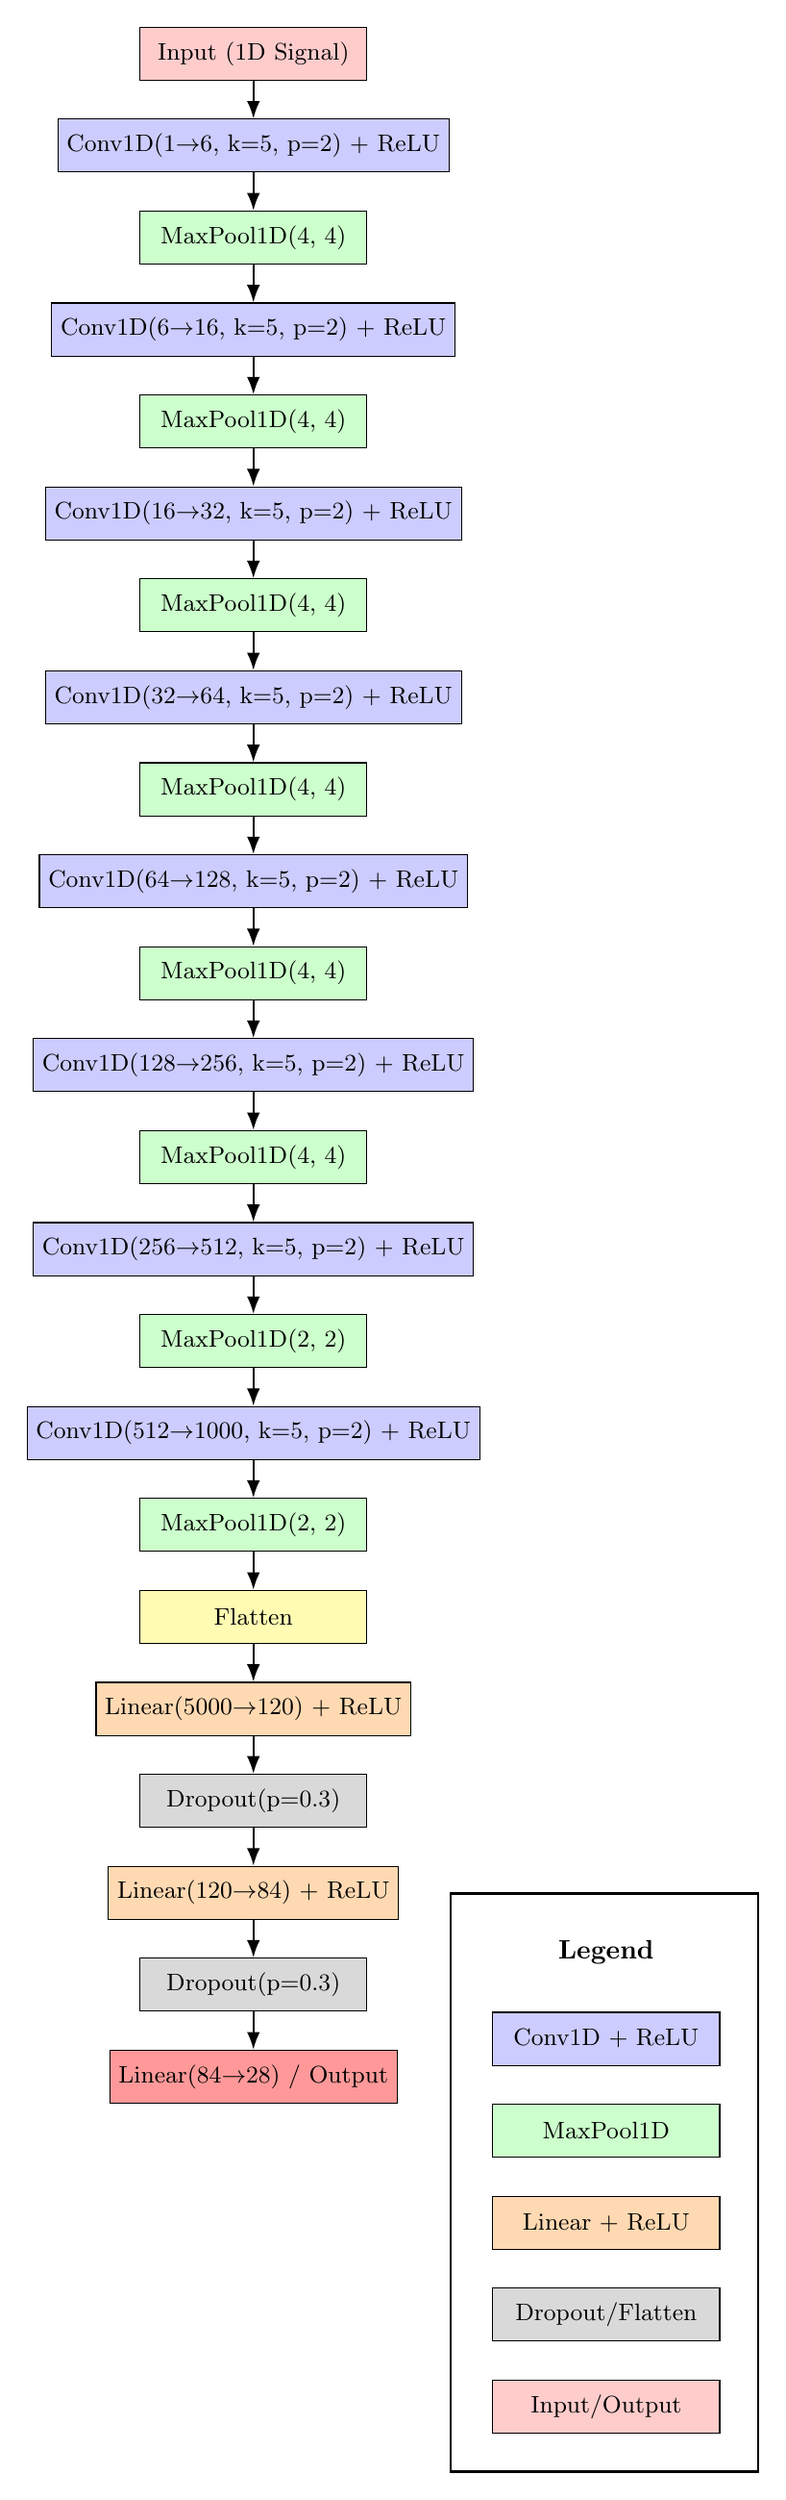
\begin{tikzpicture}[
    % 定义节点的样式
    conv/.style={rectangle, draw, fill=blue!20, minimum width=3cm, minimum height=0.7cm, align=center, font=\small},
    pool/.style={rectangle, draw, fill=green!20, minimum width=3cm, minimum height=0.7cm, align=center, font=\small},
    fc/.style={rectangle, draw, fill=orange!30, minimum width=3cm, minimum height=0.7cm, align=center, font=\small},
    other/.style={rectangle, draw, fill=gray!30, minimum width=3cm, minimum height=0.7cm, align=center, font=\small},
    arrow/.style={-Latex, thick},
    node distance=0.5cm and 1.5cm % 调整垂直和水平距离
]

% 初始输入
\node (input) [other, fill=red!20] {Input (1D Signal)};

% --- 卷积层/池化层 块 ---

% 块 1
\node (conv1) [conv, below=of input] {Conv1D(1$\to$6, k=5, p=2) + ReLU};
\node (pool1) [pool, below=of conv1] {MaxPool1D(4, 4)};

% 块 2
\node (conv2) [conv, below=of pool1] {Conv1D(6$\to$16, k=5, p=2) + ReLU};
\node (pool2) [pool, below=of conv2] {MaxPool1D(4, 4)};

% 块 3
\node (conv3) [conv, below=of pool2] {Conv1D(16$\to$32, k=5, p=2) + ReLU};
\node (pool3) [pool, below=of conv3] {MaxPool1D(4, 4)};

% 块 4
\node (conv4) [conv, below=of pool3] {Conv1D(32$\to$64, k=5, p=2) + ReLU};
\node (pool4) [pool, below=of conv4] {MaxPool1D(4, 4)};

% 块 5
\node (conv5) [conv, below=of pool4] {Conv1D(64$\to$128, k=5, p=2) + ReLU};
\node (pool5) [pool, below=of conv5] {MaxPool1D(4, 4)};

% 块 6
\node (conv6) [conv, below=of pool5] {Conv1D(128$\to$256, k=5, p=2) + ReLU};
\node (pool6) [pool, below=of conv6] {MaxPool1D(4, 4)};

% 块 7
\node (conv7) [conv, below=of pool6] {Conv1D(256$\to$512, k=5, p=2) + ReLU};
\node (pool7) [pool, below=of conv7] {MaxPool1D(2, 2)};

% 块 8
\node (conv8) [conv, below=of pool7] {Conv1D(512$\to$1000, k=5, p=2) + ReLU};
\node (pool8) [pool, below=of conv8] {MaxPool1D(2, 2)};

% --- 展平层 ---
\node (flatten) [other, below=of pool8, fill=yellow!30] {Flatten};

% --- 全连接层 块 ---

% 块 9 (FC1)
% 注意: 5000是根据输入维度推算出的展平后的特征数
\node (fc1) [fc, below=of flatten] {Linear(5000$\to$120) + ReLU};
\node (drop1) [other, below=of fc1] {Dropout(p=0.3)};

% 块 10 (FC2)
\node (fc2) [fc, below=of drop1] {Linear(120$\to$84) + ReLU};
\node (drop2) [other, below=of fc2] {Dropout(p=0.3)};

% 块 11 (Output)
% (15-1)*2 = 28
\node (output) [fc, below=of drop2, fill=red!40] {Linear(84$\to$28) / Output};


% --- 绘制箭头 ---

\draw [arrow] (input) -- (conv1);
\draw [arrow] (conv1) -- (pool1);
\draw [arrow] (pool1) -- (conv2);
\draw [arrow] (conv2) -- (pool2);
\draw [arrow] (pool2) -- (conv3);
\draw [arrow] (conv3) -- (pool3);
\draw [arrow] (pool3) -- (conv4);
\draw [arrow] (conv4) -- (pool4);
\draw [arrow] (pool4) -- (conv5);
\draw [arrow] (conv5) -- (pool5);
\draw [arrow] (pool5) -- (conv6);
\draw [arrow] (conv6) -- (pool6);
\draw [arrow] (pool6) -- (conv7);
\draw [arrow] (conv7) -- (pool7);
\draw [arrow] (pool7) -- (conv8);
\draw [arrow] (conv8) -- (pool8);
\draw [arrow] (pool8) -- (flatten);
\draw [arrow] (flatten) -- (fc1);
\draw [arrow] (fc1) -- (drop1);
\draw [arrow] (drop1) -- (fc2);
\draw [arrow] (fc2) -- (drop2);
\draw [arrow] (drop2) -- (output);


% --- 图例 (可选,增加清晰度) ---
% 定位图例标题
\node [font=\bfseries] (legend_title) [above right=1cm and 2cm of output] {Legend}; 

% 绘制图例的各个元素
\node [conv, below=0.5cm of legend_title] (legend_conv) {Conv1D + ReLU};
\node [pool, below=0.5cm of legend_conv] (legend_pool) {MaxPool1D};
\node [fc, below=0.5cm of legend_pool] (legend_fc) {Linear + ReLU};
\node [other, below=0.5cm of legend_fc] (legend_drop) {Dropout/Flatten};
\node [other, fill=red!20, below=0.5cm of legend_drop] (legend_io) {Input/Output};

% 绘制图例的边框
\coordinate (legend_tl) at ([xshift=-1.3cm, yshift=0.5cm]legend_title.north west);
\coordinate (legend_br) at ([xshift=0.5cm, yshift=-0.5cm]legend_io.south east);
\draw [thick] (legend_tl) rectangle (legend_br);

\end{tikzpicture}
\end{document}